\chapter{Results and Analysis}
\label{ch:results}
\glsresetall
\section{Preamble}

The simulation and measurement results are captured using the methods described in sections 2 and 3. A comparison between the simulation and measurement targets is completed by calculating the correlation of each targets frequency vector, at each angle. This correlation function results in a single correlation coefficient for each angle.

Generally, the correlation coefficient is below one (a perfect match between measurements). Missile 1 showed the highest correlation between its measurement and simulation, with a mean correlation coefficient of 0.862, and standard deviation of 0.092. The mean correlation of the succeeding targets decreased with each continuously, with missile 5 showing the lowest mean correlation of 0.082, and standard deviation of 0.234.

These breakdowns in correlation between measurement and simulation are expected to impact the capability of the classifier. A classifier will be considered a `failure` if it cannot exceed an accuracy of $20\%$, equivalent to randomly guessing the targets label.

\section{Measurment Results}
\label{sec:meas_res}

	Figures \ref{fig:n1}-\ref{fig:n5} represent the calibrated RCS measurements of missiles 1, 2, 3, 4, and 5 respectively. Each figure includes a plot of the vertically and horizontally polarized incident field.

	The measured values are converted to $dB_{sm}$ for the purpose of display using \ref{eq:ieee_rcs}, with a transmitted signal of $E_t = 1 [V/m^2]$, and

	\begin{equation}\label{eq:rcs_db}
		RCS [dB] = 10 * \log \left( \frac{RCS [m^2]}{1 [m^2]}\right).
	\end{equation}

	The green wedge in each RCS cut represents the \gls{AOI}, the region over which data is collected and used to train/evaluate the model. The total frequency content of each target over all angles are shown in figures \ref{fig:c1}-\ref{fig:c5}. Again, figures are shown in $RCS [\textrm{dB}_{sm}]$, and represent the calibrated RCS measurements of missiles 1-5 respectively. Each figure include a plot of the vertically and horizontally polarized incident field.

	The measurement result show a reduction in performance for all vertically polarized measurements. This is a defect in the instrumentation radar:  the amplifier bank has been experiencing deteriorated performance due to a defect in the hardware. This was known prior to  this research. HOwever, this data has been collected anyway in an attempt to utilize the results to a limited extent, as well as potentially quantify the breakdown in performance.

\section{Simulation Results}
\label{sec:sim_res}

    Figures \ref{fig:ns1}-\ref{fig:ns5} represent the simulated RCS of missiles 1-5 respectively. Each figure includes a plot of the vertically and horizontally polarized incident field.

		As with the measurement data, each plot is converted to $dB_{sm}$ using equations \ref{eq:ieee_rcs} and \ref{eq:rcs_db}.

\section{Data Comparison}
\label{sec:data_comparison}

	The angular correlation between simulated and measured targets, augmented using the normalization routine, are presented in figures \ref{fig:corr_msl1}-\ref{fig:corr_msl5}. Each figure shows the degree of correlation between one simulated target, and its correaltion with each measured target. Figures list a seperate correlation plot for horizontal and vertical polarizations.

	On examintation, Missile 1 (\ref{fig:corr_msl1}) shows the strongest autocorrelation between simulation and measurement of all targets. The autocorrelation between the simulated targets shows progressively deteriorated performance moving from missile 1 to missile 5. In fact, the measurement data for missile 1 dominates the correaltion results for missiles 2 and 3. The simulated results for missiles 2 and 3 (figures \ref{fig:corr_msl2} and \ref{fig:corr_msl3} respectrively) show stronger correaltion with missile 1, than with their own simulation. Missile 4 (figure \ref{fig:corr_msl4}) deviates from this trend, but only in the vertically polarized case. The horizontally polarized autocorrelation shows the worst performance of all models. Missile 5 shows poor autocorrelation in both polarizations. The strongest correlation for missile 5 is with missile 4's measurement data in vertical polarization.

	As a measure of correlation performance versus signal to noise ratio, the correlation per angle was recalculated with aditive noise applied to the simulation data. The average correlation product per target ($<\rho>$) over all angles is shown in figure \ref{fig:correlation_results_snr}.

	\begin{figure}[htbp!]
    \centering
    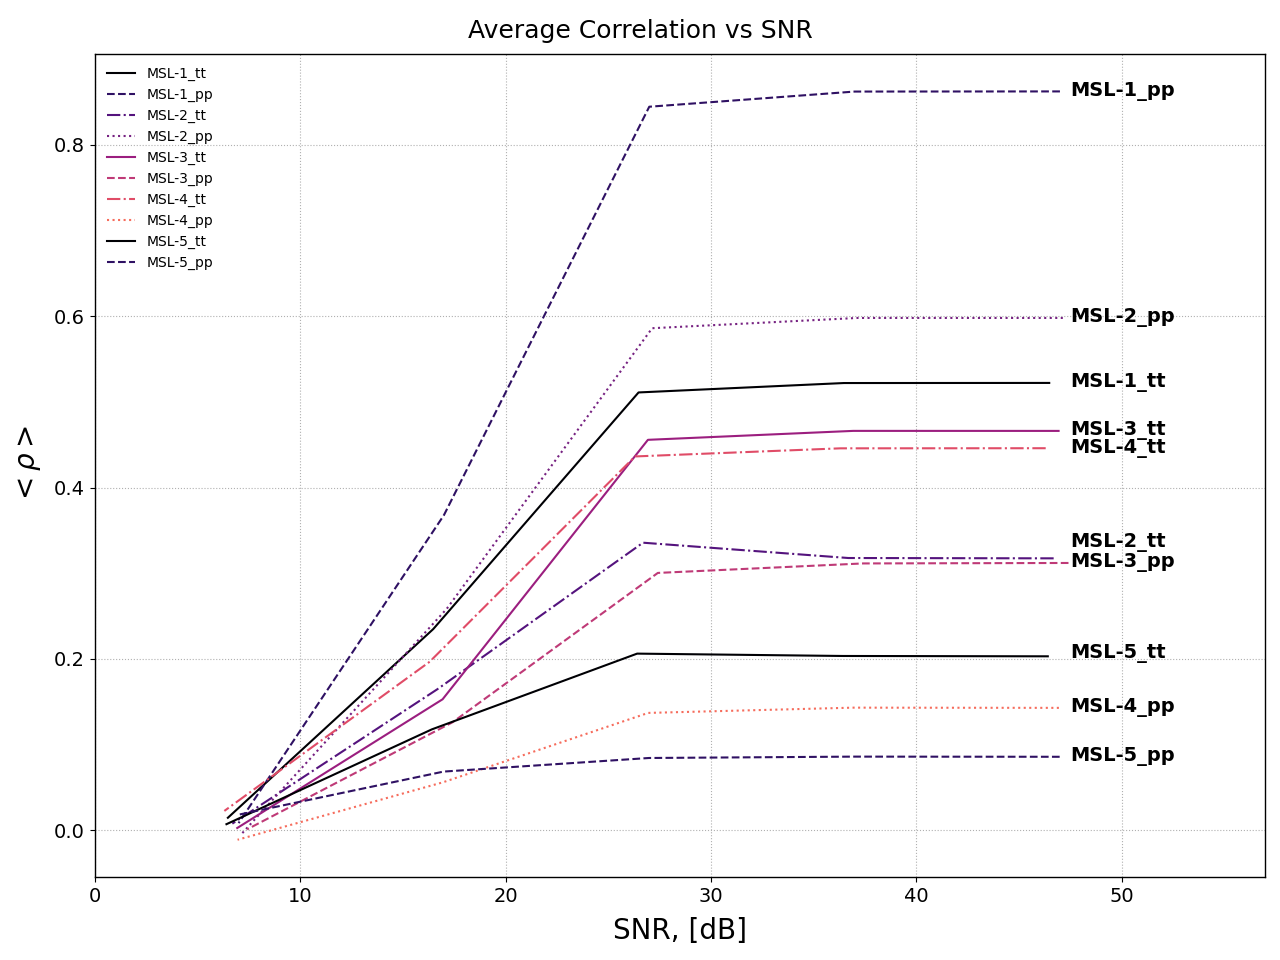
\includegraphics[width=.8\linewidth]{Correlation_vs_SNR.png}
    \caption[Average Correlation vs SNR]{Top-down and side view of the AFIT compact radar range.}
    \label{fig:correlation_results_snr}
  \end{figure}

	As expected, the average correlation between the simulated and measured data increases with SNR. At a roughly $28 dB$, correlation performance is flat. All targets show a near complete breakdown in correlation around $6 dB$. Surprisingly, the vertically polarized measurements have a higher average correlation than expected. As noted previously, correlation performance degrades for succesive targets. Missile 1's horizotnally polarized autocorrelation shows the strongest performance with an average $\rho$ of 0.892. This is followed by Missile 2's with an average $\rho$ of 0.6. The remaining measurements show a range of $<\rho>$ between 0.6 and 0.08.


\section{Model Evaluation}

	Multiple configurations were evaluated to find an optimal classifier network.

	\subsection{VGG-19}
	\label{sec:vgg-19_results}

		The VGG-19 classifier netowrk was developed by first identifying high-performing models. Model performance was determined by the calssifcation accuracy of the network for a given set of hyperparamters. Models with the highest overall accuracy were selected to be placed into a siamese network. The primary distinction of each model is the noise level that was applied to the training data. Conceptually, an array of models that have been trained on various noise levels would be able to accuractely classify a signal in the presence of random noise, similar to a contested EMOE. The noise levels applied to the VGG-19 models were $-5, 0, 5, 10$ [dBm].


		For each given noise level, models were trained and evaluated using multiple hyperparamter configurations. The list of hyperparamters, and the values they were evaluated at are show in table \ref{tab:test_factors_vgg}. The VGG-19 was only able to converge when using the SGD optimizer, which was then used for the remainder of testing. The values of momentum are applicable to the SGD optimizer only.

		Models were evaluated for their given training noise and hyperparamter configureations in ``runs.'' Each run is repeated five times to reduce statistical noise. The test results are shown in figure \ref{fig:vgg-19_performance}.

		\begin{table}[htbp!]
			\begin{center}
				\caption[Hyperparameter test factors]{List of test factors used to evaluate model performance.}
				\label{tab:test_factors_vgg}
				\begin{tabular}{|r|l|}
					\hline
					\textbf{Paramters} & \textbf{Value}\\
					\hline
					Sample size	&	1000 \\
											& 3000 \\
											& 5000 \\
					\hline
					Learning Rate	& 0.1 \\
												& 0.01 \\
												& 0.001 \\
					\hline
					Batch Size	&	100 \\
											& 200 \\
											& 300 \\
					\hline
					Optimizers	& `Adam` \\
											& `RMS Prop`\\
											& `SGD` \\
					\hline
					Momentum 	& 0.5 \\
										& 0.7 \\
										& 0.9 \\
					\hline
					Additive Noise Power 	& -20 [dBm] \\
										& -10 [dBm] \\
										& 0 [dBm] \\
										& 10 [dBm] \\
										& 20 [dBm] \\
					\hline
				\end{tabular}
			\end{center}
		\end{table}

		\begin{figure}[htbp!]
	    \centering
	    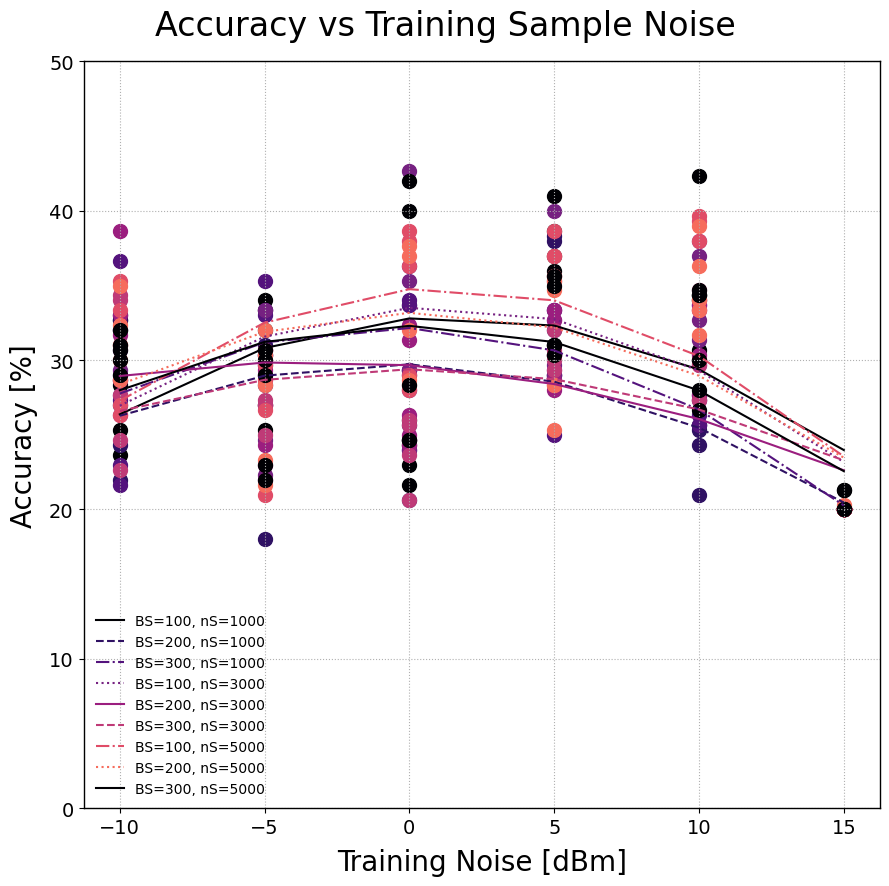
\includegraphics[width=.8\linewidth]{Acc_5000.png}
	    \caption[VGG-19 Model Testing, and Selection]{VGG-19 model performance using multiple hyperparamter configurations}
	    \label{fig:vgg_19_performance}
	  \end{figure}

		A preliminary evaluation of the listed hyperparameters was conducted to reduce the number of runs that would be required. Learning rates greater than 0.001 showed poor convergence, and resulted in failed classifications. The models using optimizers other than SGD were also unable to converge. The strongest performing models utilized a batch size of 100, and sample size of 5000.

		The top performing models were placed in siamese network, and re-evaluted using test data that has progressively large additive noise applied. The accuracy of the VGG-19 siamese network is shown in figure \ref{fig:vgg-19_siamese_results}. Here, additive noise is applied to the test data, and passed to the network for evaluation. For each noise level, the network is tested 50 times and the average accuracy is reported. The network is baselined using simulation data first, and then revaluated with measurement data. The averaged accuracy and classifier predictions are shown for each angle per SNR in figures \ref{fig:vgg-19_snr1}-\ref{fig:vgg-19_snr15}.

		\begin{figure}[htbp!]
	    \centering
	    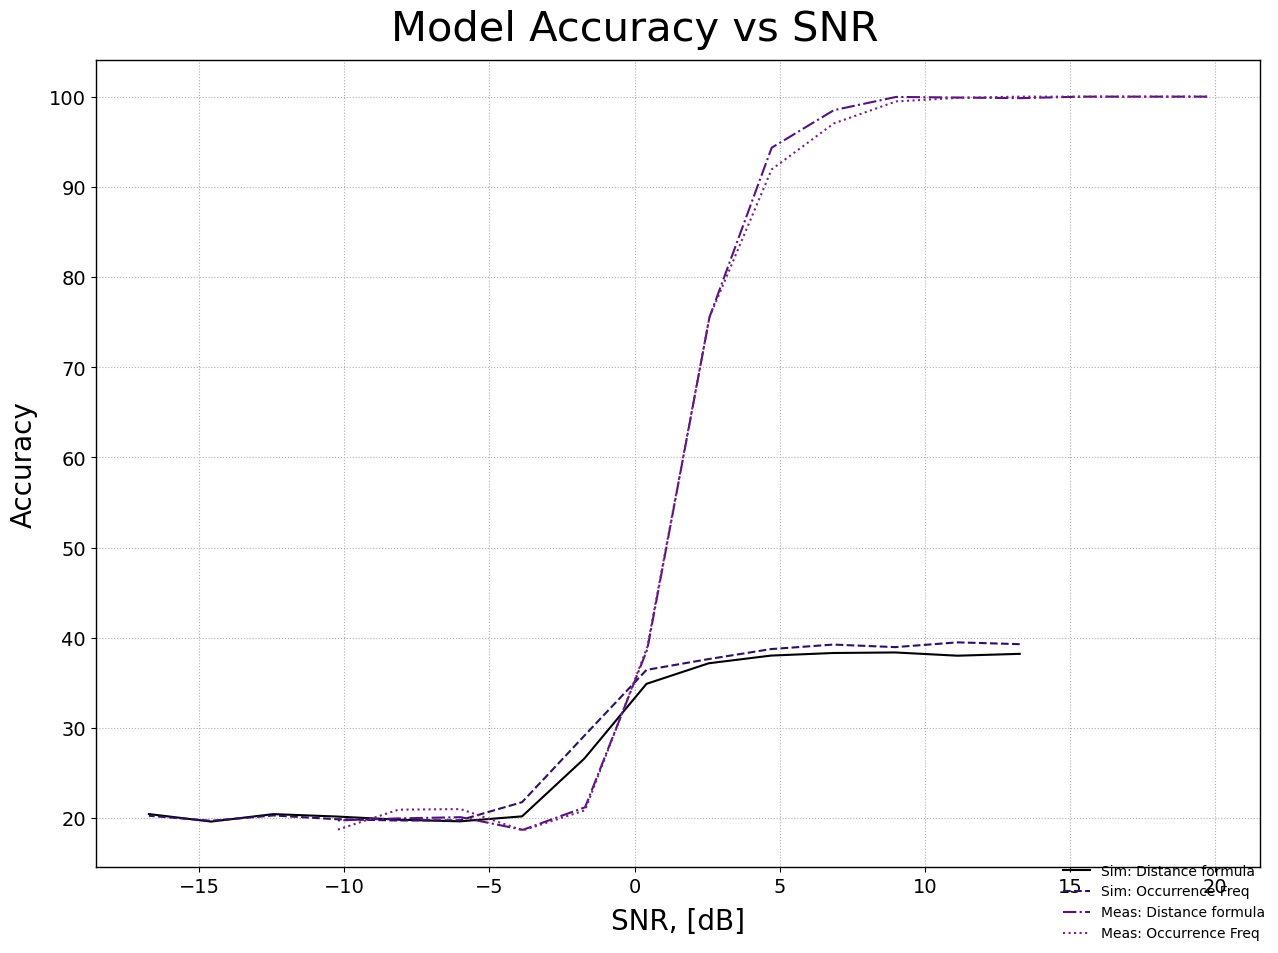
\includegraphics[width=.8\linewidth]{vgg-19_siamese_accuracy.png}
	    \caption[VGG-19 Siamese Network Performance]{VGG-19 siamese netowrk performance versus SNR}
	    \label{fig:vgg-19_siamese_results}
	  \end{figure}

		Overall, performance is low for the measurement data. This is likely due to a host of factors. As noted previosly, the autocorrelation of simulated and measured missiles breakdown for missiles 3, 4, and 5. These breakdowns are captured in the confusion matrices of each model, shown in figures \ref{fig:vgg-19_cm1}-\ref{fig:vgg-19_cm5}. The confusion matrices show a flaw in each of the models:  \textit{they tend to fixate on specific targets in order to increase evalution performance}. The most glaring example is shown in figure \ref{fig:vgg-19_cm1}. This model features the highest evalutaion performance of the group, but completely neglects missiles 3 and 5. The problem of ``fixation'' is made more galring when examing the number of classifications made by each model during their initial selection. Table \ref{tab:vgg-19_confusion_error} shows the percentage of calssifications made by each model when evaluating noiseless measurement data.

		\begin{align}
			\textrm{Missile 1:} & 48\% \notag \\ % 40 + 18 + 48 + 38
			\textrm{Missile 2:} & 33\% \notag \\ % 29 + 32 + 10 + 27
			\textrm{Missile 1:} & 9 \%\notag \\ % 0 + 5 + 11 + 11
			\textrm{Missile 1:} & 59 \% \notag \\ % 50 + 50 + 38 + 39
			\textrm{Missile 1:} & 2 \% \notag \\ % 50 + 50 + 38 + 39
		\end{align}

		In aggregate, the models favor missile 4 60\% of the time they make a classification. This result is striking considering missile 4's exceptionally weak correlation performance. This is likely due to strong correlation responses in the \textit{training data}, shown in figures \ref{fig:corr_msl1_sim}-\ref{fig:corr_msl5_sim}. There is strong cross correlation between missile 1, 2, and 3 as well as missiles 4 and 5.

		The tendency towards target fixation is further confirmed when examining figures \ref{fig:vgg-19_snr7}-\ref{fig:vgg-19_snr15}. The network latchs onto missile 4 and heavily misreports the target. This becomes more pronounced as SNR decreases.

		\subsection{VGG-16}

			The VGG-19 system's depth prevented the network from gneralizing the pararmters of the model. This is lack of generalization is suspected of creating the ``target fixation'' problem documented in the section \ref{sec:vgg-19_results}. The simplified VGG-16 model serves as a potential cure.

			The VGG-16 model was evaluted using the test matrix shown in table \ref{tab:vgg-16_test_card}. The paramters of each run were evaluted recursively in-order to reduce statistical variation in the results.



			The average performance per model versus applied training noise is shown in figure \ref{fig:vgg-16_results}. The VGG-19 siamese network utilized only the strongest performing models from each run. In the interest of increasing the networks ability to generalize, \textit{all} models generated from the runs listed in table \ref{tab:vgg-16_test_card} have been saved, and used to construct the network.

			\begin{figure}[htbp!]
		    \centering
		    \includegraphics[width=.8\linewidth]{acc_2000.png}
		    \caption[VGG-19 Siamese Network Performance]{VGG-16 model performance.}
		    \label{fig:vgg-16_results}
		  \end{figure}
